% !TEX root = ../../thesis.tex

\documentclass[../../thesis.tex]{subfiles}
 
\begin{document}

In this chapter, we experiment our solvers and discuss the results. 

\section{Benchmark process}

Our benchmark API takes an options structure (\autoref{benchmark:options}).
The arrays \texttt{T}, \texttt{D} and \texttt{W} determines the sizes of the instances. The benchmark runner 
will create instances with a combinations of those parameters. For example, with the values in \autoref{benchmark:options},
the benchmark runner will create 6 instances with the sizes: $(5, 30, 100)$, $(5, 50, 100)$, $(5, 30, 200)$, $(5, 50, 200)$, $(5, 30, 300)$ and $(5, 50, 300)$ with the 
three values being $(T, D, W)$.

\begin{lstlisting}[style=scalaStyle,label={benchmark:options},caption={Benchmark options},captionpos=b]
trait BenchmarkOptions {
  val solutionLimit: Int = Int.MaxValue
  val timeLimit: Int = 20
  val repeat: Int = 1
  val dryRun: Int = 1
  val T: Array[Int] = Array(5)
  val D: Array[Int] = Array(30, 50)
  val W: Array[Int] = Array(100, 200, 300)
  val probabilities: Map[String, Double] = Map()
  val seed: Long = -1L
}
\end{lstlisting}

We can specify a solution limit as well as a time limit. We can also repeat our benchmark and takes 
the average of results. We can also have dry runs to warm up the JVM (Java Virtual Machine) and a seed to have reproducible benchmarks. Finally,
we can specify the probabilities for our instances as explained in \autoref{section:instance-gen}.

Our benchmark runner has a function \texttt{run} that takes a name (e.g. solver name, serie name, etc), and a solving function 
which takes a generic model and returns a pair with the time spent in milliseconds and the objective value respectively.

\begin{lstlisting}[style=scalaStyle,label={benchmark:run},caption={Benchmark run function},captionpos=b]
class BenchmarkRunner(val options: BenchmarkOptions) {
  def run (
    name: String, 
    solve: VillageOneModel => (Long, Int)
  ): (BenchmarkSerie, BenchmarkSerie)
}
\end{lstlisting}

This functions returns a pair of benchmark series: one serie for the time values and one serie for the objective values.
The \texttt{BenchmarkSerie} class is simply a class that takes a name and a list of benchmark measurements (i.e. mean, standard deviation, min and max).

This implementation allows us to create a variety of benchmark by simply changing the \texttt{solve} function.


\section{Constraint Programming}

\subsection{Heuristics}

\autoref{experiments:heuristic1} shows the objective ratio between the implemented custom \textit{Most Available} Heuristic and a standard 
\textit{First Fail} heuristic after the first solution. The two heuristics were tested on 72 instances of various sizes from small to big instances.
The performance profile shows a gain of about $2$ to $3.4$ for our custom heuristic.


\begin{figure}
  \centering
  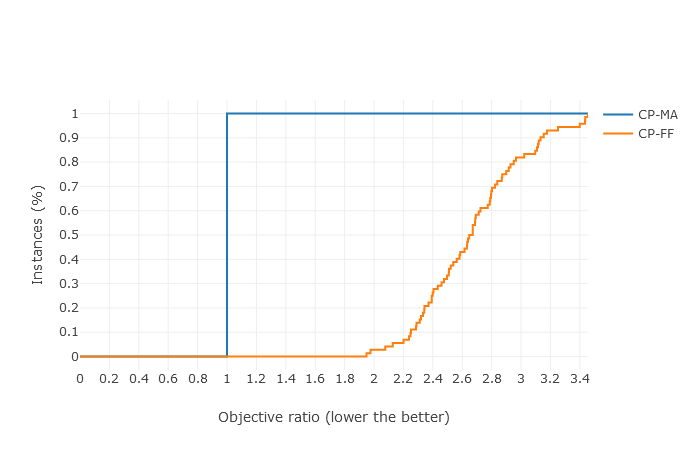
\includegraphics[scale=0.55]{experiments/heuristic.png}
  \caption{Most Available and First Fail heuristics [72 instances/first solution].}
  \label{experiments:heuristic1}
\end{figure}

\begin{figure}
  \centering
  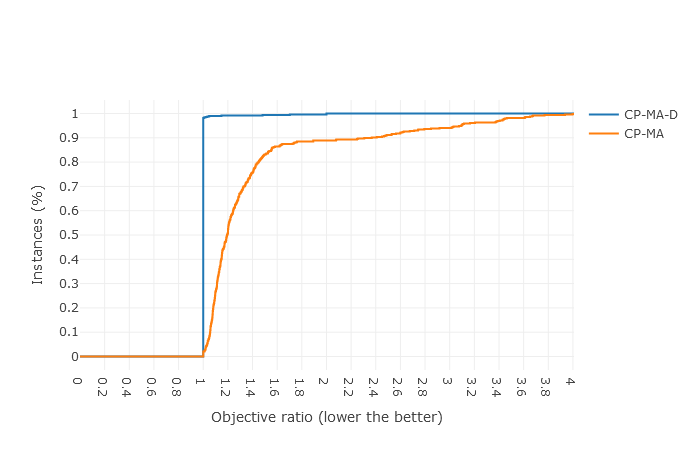
\includegraphics[scale=0.55]{experiments/static-dynamic-heuristic.png}
  \caption{Most Available: static and dynamic [486 instances/15s].}
  \label{experiments:heuristic2}
\end{figure}


\subsection{Large Neighborhood Search}


\section{Comparing solvers}

We now start by comparing different solvers together. \autoref{experiments:solvers:3} 
shows a performance profile generated from 216 instances of various sizes.
This benchmark was set to a time limit of 30s per instance. The baseline of this 
profile is the CP solver. We observe that the CP solver performs better than MIP in more than 80\% of instances.
However, we also tested the MIP solver by giving it a first solution obtained from CP, we can see that it slightly outperforms CP and MIP in 80\% of instances.

\begin{figure}
  \centering
  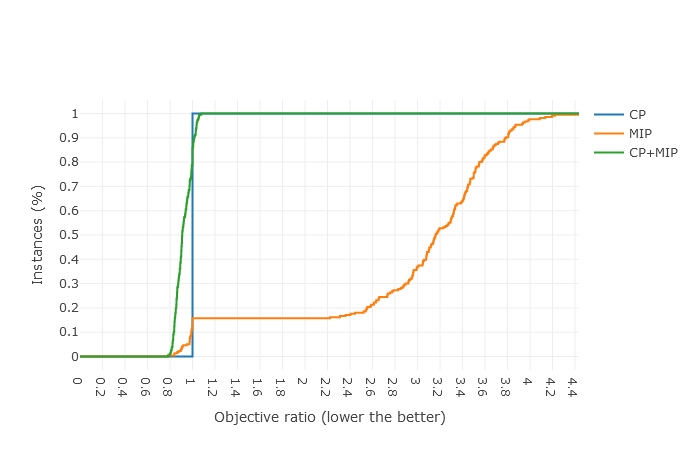
\includegraphics[scale=0.55]{experiments/solvers.png}
  \caption{CP, MIP and CP+MIP solvers [216 instances/30s].}
  \label{experiments:solvers:3}
\end{figure}


\begin{figure}
  \centering
  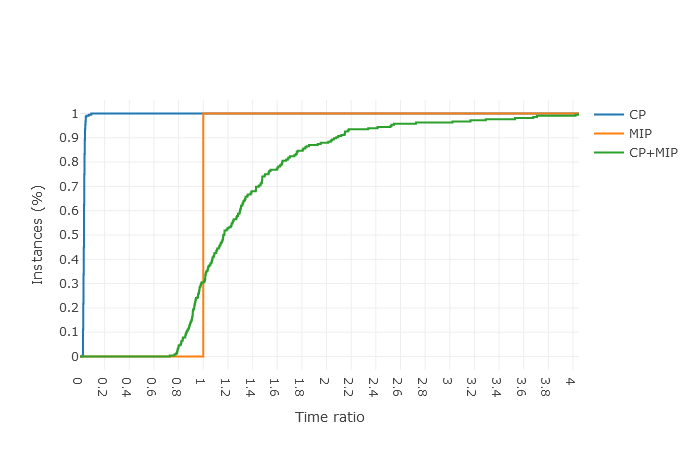
\includegraphics[scale=0.55]{experiments/time-first-sol.png}
  \caption{Time on first solution [216 instances/First solution].}
  \label{experiments:first-sol-time}
\end{figure}


\begin{figure}
  \centering
  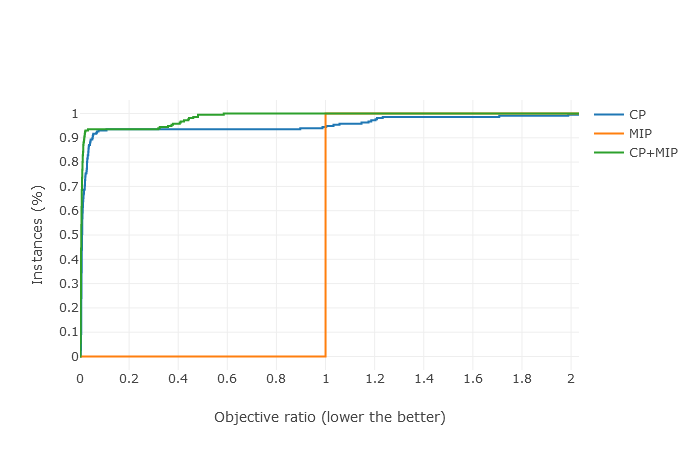
\includegraphics[scale=0.55]{experiments/obj-first-sol.png}
  \caption{Objective on first solution [216 instances/First solution].}
  \label{experiments:first-sol-obj}
\end{figure}




\end{document}

